% This is a semi-simple sample document.

\documentclass{article} % \documentclass{} is the first command in any LaTeX code.  It is used to define what kind of document you are creating such as an article or a book, and begins the document preamble

%\usepackage[spanish]{babel} % Para traducir palabras claves al español como "Figure" -> "Figura"

\usepackage{amsmath, amssymb} % \usepackage is a command that allows you to add functionality to your LaTeX code

\usepackage{mathtools} % using cases inside equations

\usepackage{graphicx} % image package

\usepackage{float} % Float specifiers are written in the square brackets whenever we use a float such as a figure or a table

\usepackage{subcaption} % more than one picture s in the same figure

\parskip 0.1in %paragraph distance

\usepackage[margin=0.984252in]{geometry} %margin

\usepackage[hidelinks]{hyperref} % Magic for index linking

\usepackage{chngcntr} % For figure number matching with section number
\counterwithin{figure}{section}

\usepackage{appendix} % Appendix

\usepackage{listings} % Para display codigo

\title{Trabajo Práctico N°1} % Sets article title
\date{Septiembre 2023} % Sets article date

\author{
	\textbf{Fundamentos de Análisis de Datos}\\
	Maestría en Ciencia de Datos\\
	\\~\\
	\textbf{Estudiantes: }\\
	\textbf{Ing. Flores, Matías Gabriel}\\
	matflores@itba.edu.ar
 	\\~\\
 	\textbf{Ing. Loiseau, Matías}\\
 	mloiseau@itba.edu.ar
 	\\~\\
	\textbf{Docente: }\\
	\textbf{Dra. Rey, Andrea A.}
}

% The preamble ends with the command \begin{document}
\begin{document} % All begin commands must be paired with an end command somewhere

\begin{figure}
\centering
	
\includegraphics[width=0.2\textwidth]{images/itba-logo}
	%\caption{Mi Figure}
	\label{fig:itba-logo}
\end{figure}
\maketitle % creates title using information in preamble (title, author, date)

\thispagestyle{empty} % Ignore page number
\cleardoublepage

\cleardoublepage
\tableofcontents % general index
\cleardoublepage


\section{Ejercicio N° 1}

En el archivo \textit{Dieta.xlsx} se encuentran los datos correspondientes a 173 personas que están siguiendo una dieta. Para cada una de ellas, se registró el sexo y el consumo de grasas saturadas y de alcohol, así como del total de calorías diarias.

\subsection{Primer punto}

\textbf{Consigna:} Analizar si existen datos faltantes y, en caso afirmativo, eliminar tales registros.

Antes de empezar con la consigna, debemos aclarar que previo al análisis, cargamos las librerías necesarias y el dataset en un data frame llamado \textit{Dieta}.

Para analizar si existen datos nulos utilizamos dos funciones en específico 	que nos sirven para determinar las posiciones en donde se encuentran dichos datos. Para verificar si los datos fueron borrados correctamente, contamos la cantidad de filas antes y después de ejecutar la función de borrado. 

La cantidad de filas del data frame era de 173, y la función devolvió que las posiciones donde los datos eran nulos fueron: 172, 195, 198 y 336 (donde el máximo valor era $173 x 4$). Luego de aplicar la función de borrado, quedaron 169 filas, convirtiéndose en un data frame limpio para ser analizado.

\subsection{Segundo punto}

\textbf{Consigna:} Calcular las siguientes medidas estadísticas descriptivas clásicas del consumo de grasas: rango, media, mediana, desvío estándar y rango intercuartil.

En la tabla 1 se pueden apreciar las medidas estadísticas descriptivas de todas las variables cuantitativas del dataset Dieta. Creemos pertinente agregar las variables Alcohol y Calorías al análisis ya que aporta una visión más general del dataset.

\begin{table}[H]
	\centering
		\begin{tabular}{||l || c | c | c | c | c ||}
			\hline
			\hline
			Variable & Rango & Media & Mediana & Desvío Estándar & Rango Intercuartil\\
			\hline			
			\hline
			Grasas & 11.82 - 46.36 & 24.59 & 24.09 & 6.40 & 7.95\\
			\hline
			Alcohol & 0.00 - 40.11 & 8.66 & 5.84 & 8.94 & 11.19\\
			\hline
			Calorías & 900 - 2376 & 1585.44 & 1585 & 291.43 & 355\\
			\hline
			\hline
		\end{tabular}
		\caption{Medidas descriptivas de las variables del dataset Dieta.}
	\label{tab:table-punto-1-2}
\end{table}

\subsection{Tercer punto}

\textbf{Consigna:} Realizar gráficos boxplots de los datos sobre el consumo de calorías en función de la variable categórica. ¿Qué puede observarse?

En la figura 1.1 se encuentra graficado el boxplot a partir de los datos de la tabla 2. Podemos observar que ambas cajas son bastante similares, pero el consumo de calorías de los hombres se encuentra levemente más dispersa que el de las mujeres. 

La segunda diferencia notoria es que la mediana en los hombres está centrada a la misma distancia entre los cuartiles Q1 y Q3, mientras que en el caso de las mujeres la mediana se encuentra más cerca al tercer cuartil.

Ademas, se puede ver que los limites para el caso masculino son mas abarcativos, teniendo un rango mas amplio. Por último, se observa que ambos conjuntos de datos contienen dos valores atípicos. 

\begin{table}[H]
	\centering
		\begin{tabular}{||l || c | c | c | c | c | c ||}
			\hline
			\hline
			Sexo & Min & 1er Q & Mediana & Media & 3er Q  & Max\\
			\hline			
			\hline
			Masculino & 923 & 1429 & 1598 & 1628 & 1783 & 2376\\
			\hline
			Femenino & 900 & 1400 & 1583 & 1551 & 1721 & 2013\\
			\hline
			\hline
		\end{tabular}
		\caption{Medidas descriptivas de Calorías según Sexo.}
	\label{tab:table-punto-1-3}
\end{table}

\begin{figure}[H]
	\centering
	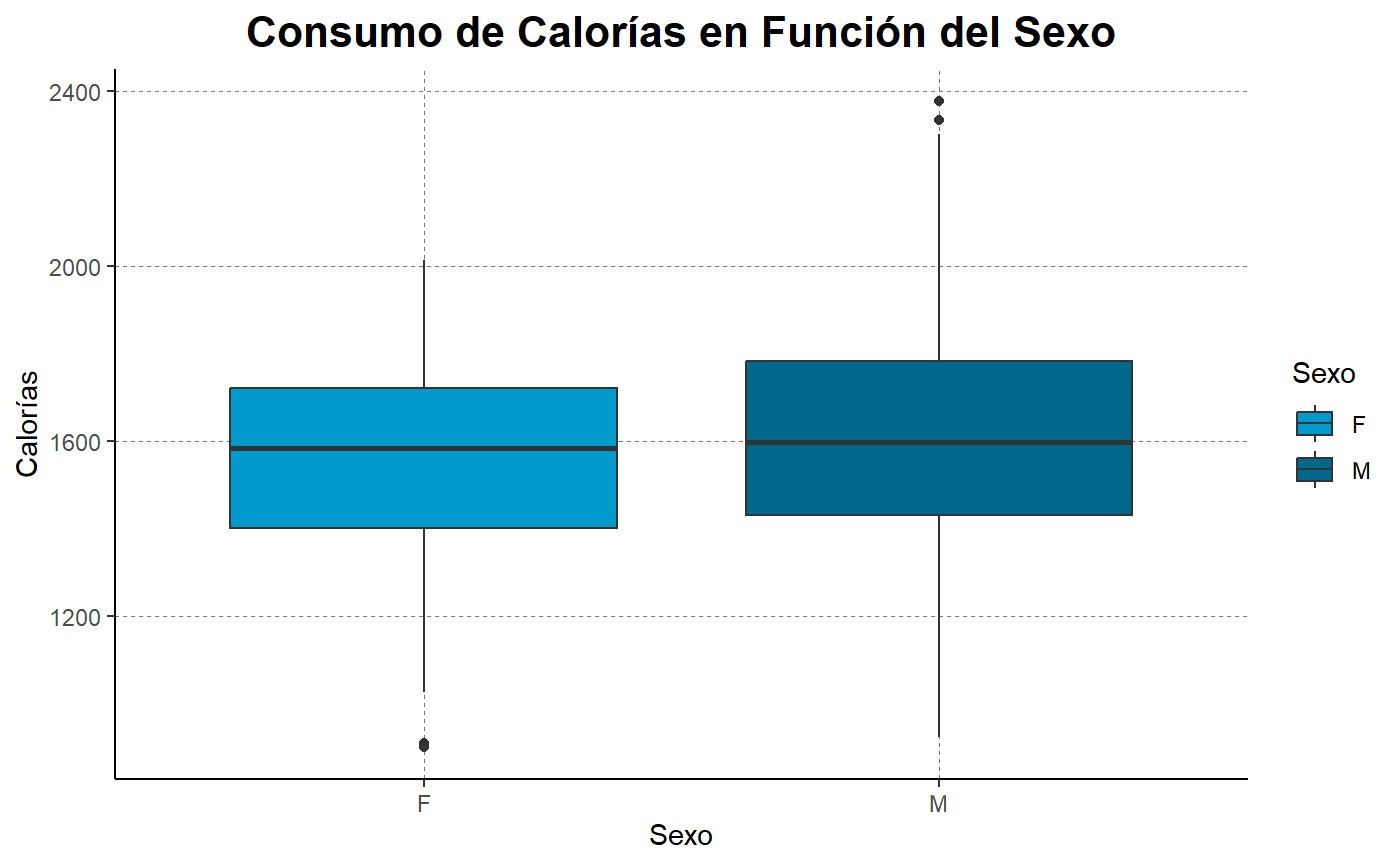
\includegraphics[width=0.8\textwidth]{images/1-3 Boxplot}
	\caption{Boxplot de Consumo de Calorías en Función del Sexo.}
	\label{fig:boxplot1}
\end{figure}

\subsection{Cuarto punto}

\textbf{Consigna:} Dividir la cantidad de calorías consumidas en dos categorías: MODERADA (menor o igual a 1700) o ALTA (mayor a 1700). Analizar el consumo de alcohol de acuerdo a la cantidad de calorías consumidas según las categorías definidas.

En primer lugar, creamos dos data frames en base a la cantidad de calorías consumidas, para poder realizar un mejor análisis de cada una por separado. Lo primero que podemos observar es que para la categoría moderada quedaron 117 registros, mientras que para la categoría alta fueron 52, siendo casi la mitad de la otra, visualizado en la tabla 3.

\begin{table}[H]
	\centering
		\begin{tabular}{||l | c ||}
			\hline
			\hline
			Categoría & 	Filas\\
			\hline			
			\hline
			Alta & 52\\
			\hline
			Moderada & 117\\
			\hline
			\hline
		\end{tabular}
		\caption{Cantidad de filas para ambas categorías.}
	\label{tab:table-punto-1-4}
\end{table}

Luego, decidimos gráficar los valores de cada uno en distintos gráficos, por lo cual hicimos un histograma sobre el consumo de alcohol para cada categoría, figuras 1.2 y 1.3. Para visualizar correctamente la distribución de la variable, realizamos el cálculo de 3 bins. Los métodos elegidos fueron Sturges, Scott y Freedman-Diaconis. Para ambos casos seleccionamos el método de Sturges.

\begin{figure}[H]
	\centering
	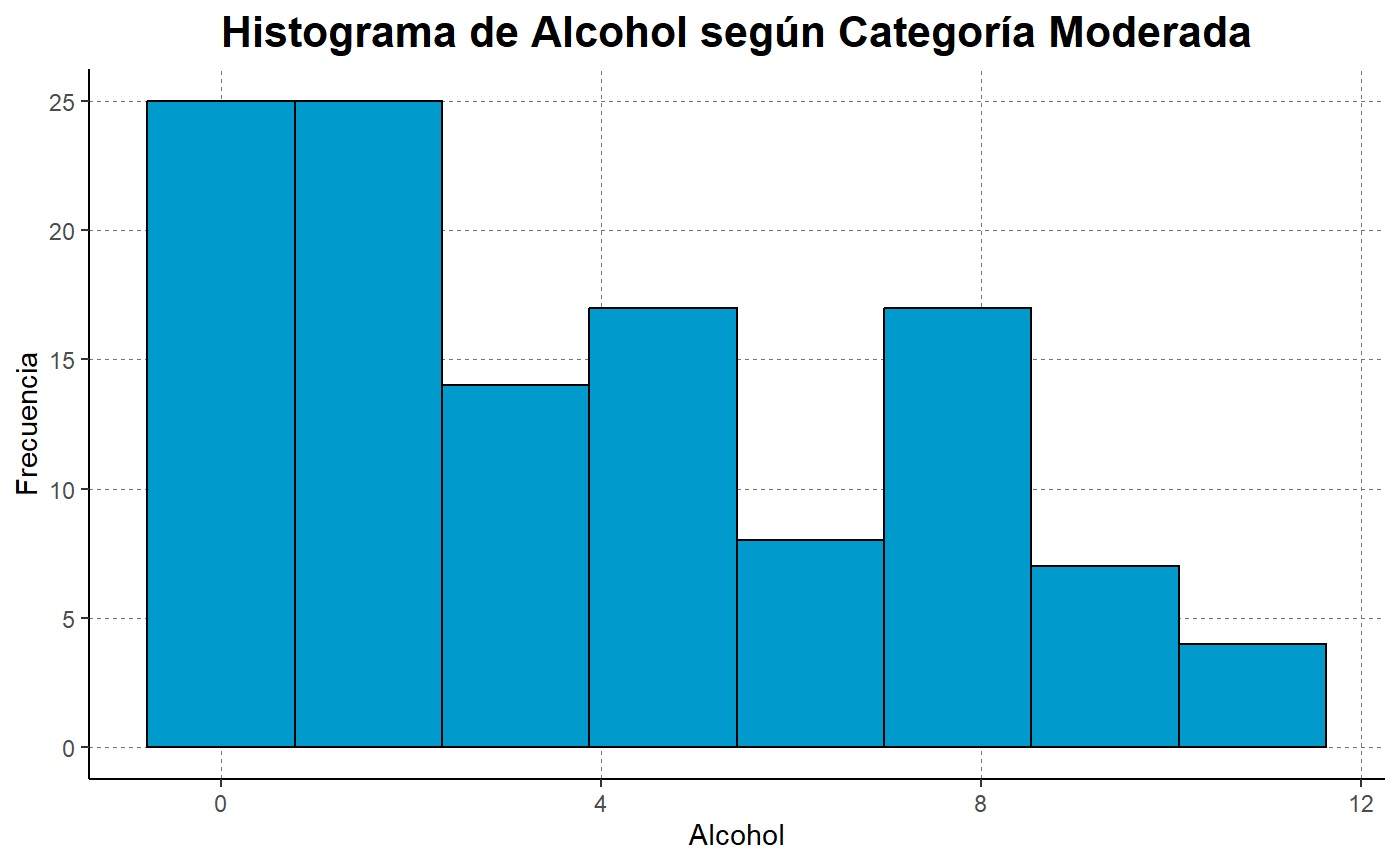
\includegraphics[width=0.8\textwidth]{images/1-4 hist 1}
	\caption{Histograma de Alcohol según Categoría Moderada.}
	\label{fig:hist1}
\end{figure}

\begin{figure}[H]
	\centering
	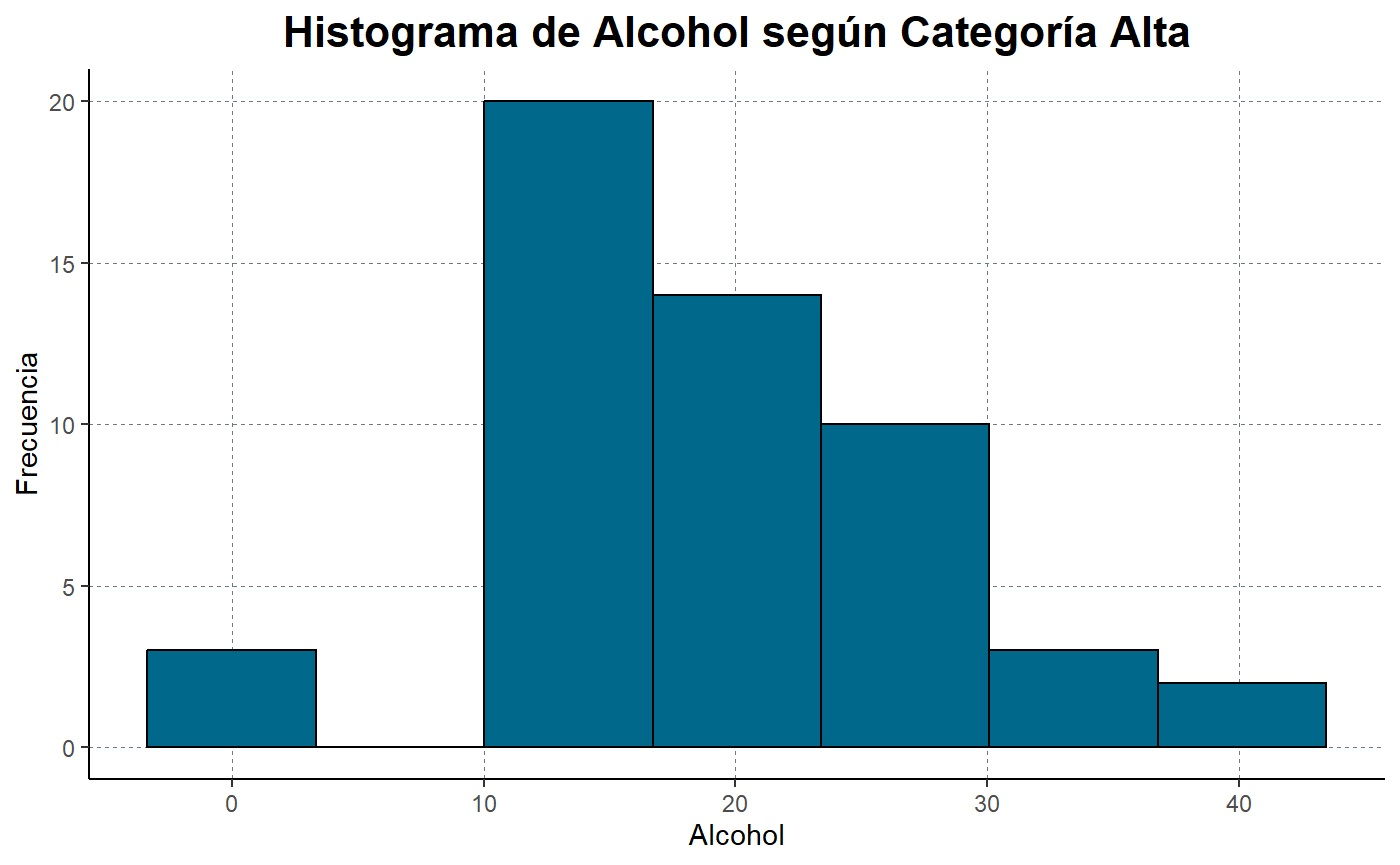
\includegraphics[width=0.8\textwidth]{images/1-4 hist 2}
	\caption{Histograma de Alcohol según Categoría Alta.}
	\label{fig:hist2}
\end{figure}

Para ambos casos, a simple vista no se puede observar un supuesto de normalidad concreto. Además, se ve que en la categoría moderada el consumo de alcohol no llega a 12, por otro lado para el caso de alta llega a valores cercanos a 40.

Para el caso de moderada, se puede apreciar que hay una mayor distribución entre el 0 y el 12, estando más concentrado en valores cercanos a 0; en cambio en la otra categoría la mayor distribución de datos se encuentra a partir del valor 10, teniendo una mayor concentración en los valores centrales.

Después, decidimos realizar un boxplot de cada categoría para poderlas analizar en mas detalle. Visto en la figura 1.4, gráficado a partir de los datos de la tabla 4.

\begin{table}[H]
	\centering
		\begin{tabular}{||l || c | c | c | c | c | c ||}
			\hline
			\hline
			Categoría & Min & 1er Q & Mediana & Media & 3er Q  & Max\\
			\hline			
			\hline
			Moderada & 0 & 0.85 & 3.35 & 3.94 & 6.9 & 10.8\\
			\hline
			Alta & 0 & 13.75 & 17.8 & 19.2 & 24.4 & 40.11\\
			\hline
			\hline
		\end{tabular}
		\caption{Medidas descriptivas de Alcohol según Categoría.}
	\label{tab:table2-punto-1-4}
\end{table}

\begin{figure}[H]
	\centering
	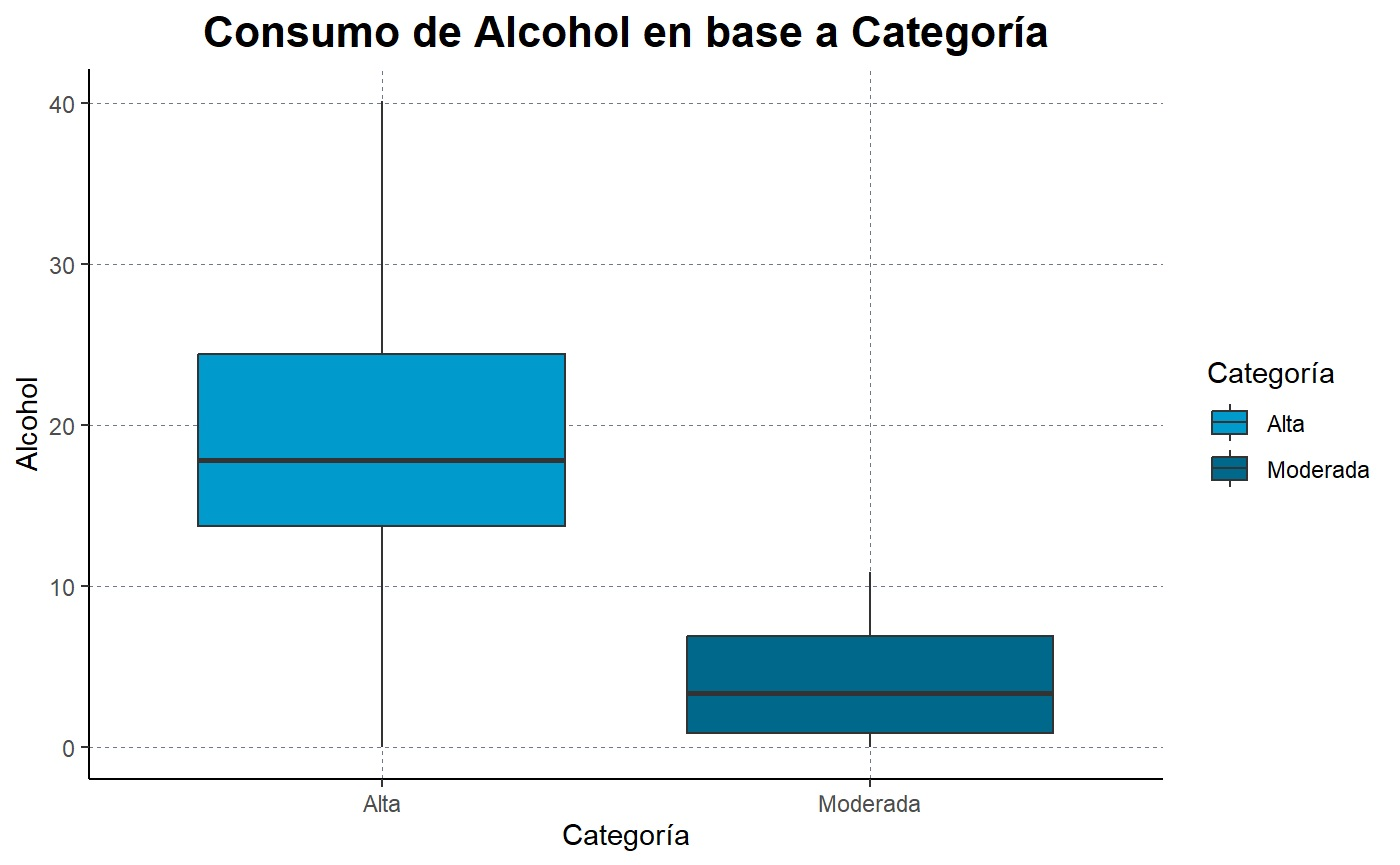
\includegraphics[width=0.8\textwidth]{images/1-4 box}
	\caption{Boxplot de Consumo de Alcohol en base a Categoría.}
	\label{fig:box2}
\end{figure}

En la figura 1.4 se aprecia que el consumo de alcohol para la categoría alta tiene una mayor cantidad de dispersión que la moderada. Además, podemos confirmar que las personas con mayor consumo de calorías son también aquellas que consumen más alcohol. 

A partir de estos datos, podemos verificar que las personas que se encuentran en la categoría alta, tienen un consumo de alcohol mas amplio que va desde 0 hasta 40, en contraste a la moderada que llega a 10. Ademas, la mayor concentración del consumo de alcohol para el caso alta se encuentra en valores mucho mas superiores a los de la categoría moderada. Por ultimo, cabe destacar que ninguna de las dos categorías presenta valores atípicos.


\section{Ejercicio N° 2}
El archivo \textit{Sociodemograficos.xlsx} contiene datos sobre distintos indicadores socio-demográficos de varios países.

\subsection{Primer punto}

\textbf{Consigna:} ¿Cuáles son las variables de interés? ¿Cuántos países fueron analizados?

Las variables de interés son: Tasa de natalidad, Tasa de mortalidad, Tasa de mortalidad infantil, Tasa de personas mayores de 65 años, Expectativa de vida al nacer, Expectativa de vida al nacer en varones, Expectativa de vida al nacer en mujeres y Población urbana. Fueron analizados 26 países.

\subsection{Segundo punto}

\textbf{Consigna:} ¿Cuáles son los países con menor y mayor tasa de natalidad?

El país con menor tasa de natalidad es Austria con 9. En cambio, el país con mayor tasa de natalidad es Afganistán con 47. 

\subsection{Tercer punto}

\textbf{Consigna:} Realizar un diagrama de dispersión con las tasas de natalidad y de mortalidad infantil. ¿Qué puede observarse? Justificar lo observado a partir del gráfico con una medida cuantitativa.

\begin{figure}[H]
	\centering
	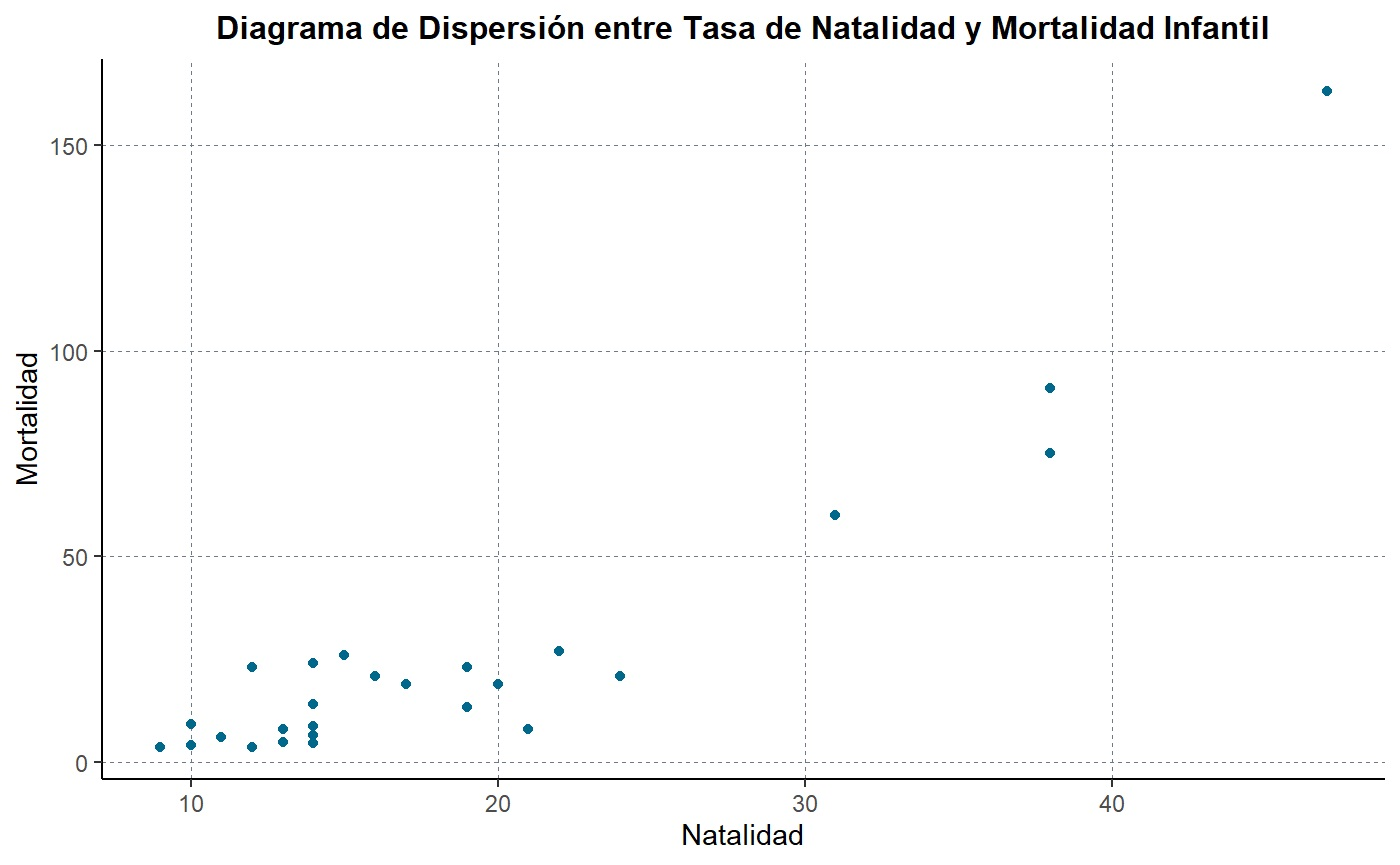
\includegraphics[width=0.8\textwidth]{images/2-3 scatter}
	\caption{Diagrama de Dispersión entre Tasa de Natalidad y Mortalidad Infantil.}
	\label{fig:scatter1}
\end{figure}

En el diagrama de dispersión de la figura 2.1, podemos observar que la mayor concentración de países se encuentra en la parte inferior izquierda de la figura. Además, se visualiza un patrón lineal, que va en crecimiento hacia el lado derecho del gráfico, por lo cual podemos observar una fuerte relación entre la tasa de natalidad y de mortalidad infantil. El valor de esta correlación se puede analizar con la correlación de Pearson. En este caso nos dio un valor de $0.9198$, lo cual quiere decir que existe una correlación positiva fuerte entre ambas tasas.

\subsection{Cuarto punto}

\textbf{Consigna:} Calcular el vector de medias y medianas.

En la tabla 5 se muestra las medias y medianas de todas las variables.

\begin{table}[H]
	\centering
		\begin{tabular}{||l || c | c ||}
			\hline
			\hline
			Variable & Media & Mediana\\
			\hline			
			\hline
			Tasa de Natalidad & 18.73 & 14.50\\
			\hline
			Tasa de Mortalidad & 8.84 & 8.00\\
			\hline
			Tasa de Mortalidad infantil & 26.42 & 16.50\\
			\hline
			Tasa de personas mayores de 65 años & 8.84 & 8.00\\
			\hline
			Expectativa de vida al nacer & 70.81 & 73.00\\
			\hline
			Expectativa de vida al nacer en varones & 68.31 & 71.00\\
			\hline
			Expectativa de vida al nacer en mujeres & 73.35 & 76.00\\
			\hline
			Población urbana & 45333423 & 8673000\\
			\hline
			\hline
		\end{tabular}
		\caption{Media y Mediana de cada una de las variables del set de datos.}
	\label{tab:table-punto-2-4}
\end{table}

\subsection{Quinto punto}

\textbf{Consigna:} Calcular las matrices de covarianzas y de correlaciones. A partir de estas matrices dar un ejemplo de dos variables fuertemente correlacionadas positivamente, de dos variables fuertemente correlacionadas negativamente y de dos variables no correlacionadas.

En la tabla 6 se visualiza la matriz de covarianzas, mientras que en la figura 2.2, la matriz de correlaciones. 

\begin{table}[H]
	\centering
		\begin{tabular}{||l || c | c | c | c | c | c | c | c ||}
			\hline
			\hline
			Variable & T. Nat. & T. Mort. & T. Mort. i. & T. 65 & Exp. vida & Exp. V & Exp. M & P. urb.\\
			\hline			
			\hline
			T. Nat. & $9.34e^{1}$ & $2.31e^{1}$ & $3.15e^{2}$& $-3.49e^{1}$ & $-8.87e^{1}$ & $-8.02e^{1}$ & $-9.63e^{1}$ & $-2.22e^{8}$\\
			\hline
			T. Mort. & $2.31e^{1}$ & $2.27e^{1}$ & $1.08e^{2}$& $6.55e^{-1}$ & $-4.05e^{1}$ & $-3.95e^{1}$ & $-4.25e^{1}$ & $-6.80e^{7}$\\
			\hline
			T. Mort. i. & $3.15e^{2}$ & $1.08e^{2}$ & $1.25e^{3}$& $-1.02e^{2}$ & $-3.31e^{2}$ & $-3.04e^{2}$ & $-3.58e^{2}$ & $-3.75e^{8}$\\
			\hline
			T. 65 & $-3.49e^{1}$ & $6.55e^{-1}$ & $-1.02e^{2}$& $2.40e^{1}$ & $3.06e^{1}$ & $2.63e^{1}$ & $3.38e^{1}$ & $2.65e^{7}$\\
			\hline
			Exp. vida & $-8.87e^{1}$ & $-4.05e^{1}$ & $-3.31e^{2}$& $3.06e^{1}$ & $1.17e^{2}$ & $1.09e^{2}$ & $1.25e^{2}$ & $1.582e^{8}$\\
			\hline
			Exp. V & $-8.02e^{1}$ & $-3.95e^{1}$ & $-3.04e^{2}$& $2.63e^{1}$ & $1.09e^{2}$ & $1.04e^{2}$ & $1.16e^{2}$ & $1.63e^{8}$\\
			\hline
			Exp. M & $-9.63e^{1}$ & $-4.25e^{1}$ & $-3.58e^{2}$& $3.38e^{1}$ & $1.25e^{2}$ & $1.16e^{2}$ & $1.34e^{2}$ & $1.52e^{8}$\\
			\hline
			P. urb. & $-2.22e^{8}$ & $-6.80e^{7}$ & $-3.75e^{8}$& $2.65e^{7}$ & $1.58e^{8}$ & $1.63e^{8}$ & $1.52e^{8}$ & $1.47e^{16}$\\
			\hline
			\hline
		\end{tabular}
		\caption{Matriz de Covarianzas Sociodemograficos.}
			\label{tab:table-punto-2-5}
\end{table}

\begin{figure}[H]
	\centering
	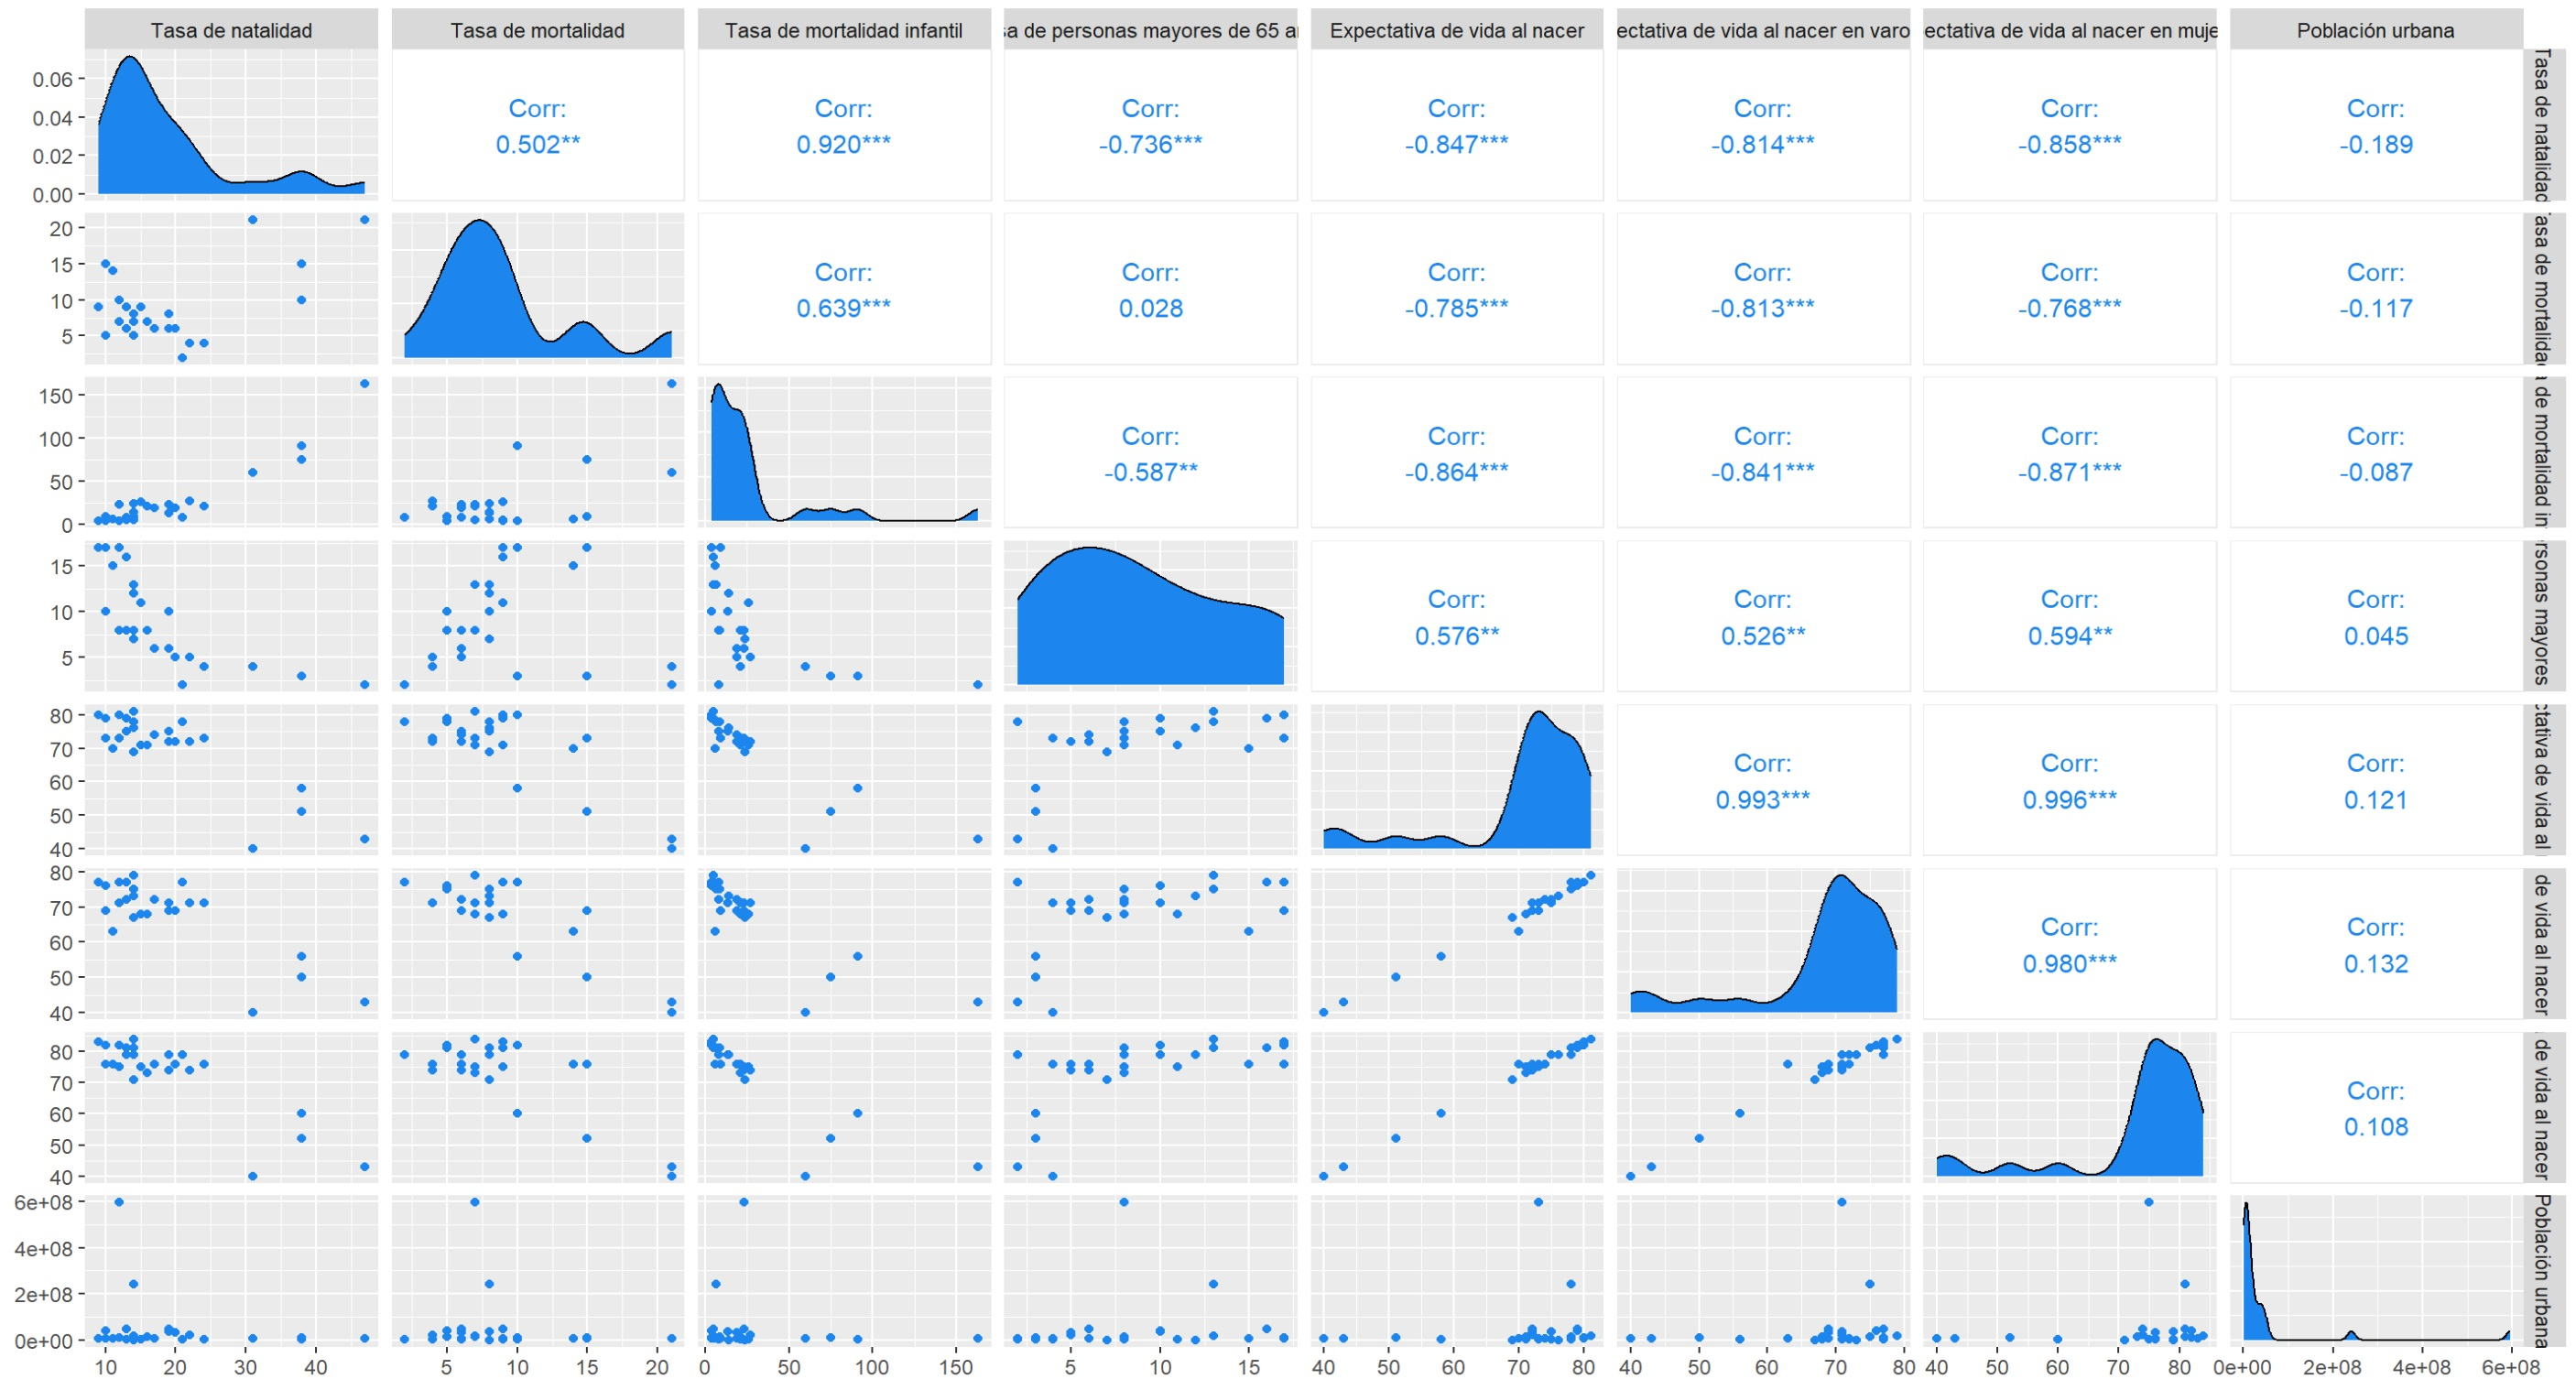
\includegraphics[width=1\textwidth]{images/2-5 corr}
	\caption{Matriz de Correlaciones Sociodemograficos.}
	\label{fig:corr1}
\end{figure}

A partir de estos datos, observamos que las variables de expectativa de vida al nacer y la expectativa de vida al nacer en mujeres tienen una fuerte correlación positiva. En cambio, la expectativa de vida al nacer en mujeres con la tasa de mortalidad infantil tienen una fuerte correlación negativa. Por último, podemos ver que no existe correlación alguna entre la tasa de personas mayores a 65 años y tasa de mortalidad.

\section{Ejercicio N° 3}
Vamos a considerar el conjunto de datos \textit{swiss} disponible en R.

\subsection{Primer punto}

\textbf{Consigna:} Cargar la base de datos y explorarla. ¿Cuántos registros y cuántas variables tiene? Describir las variables de estudio.

A partir del análisis del dataset podemos determinar que tiene 47 registros correspondientes a las provincias de suiza y 6 variables de estudio. Las mismas son: fertilidad, agricultura, examinación, educación, catolicismo y mortalidad infantil. Todas las variables se encuentran en porcentajes. En la tabla 7 se pueden visualizar las variables con sus descripciones.

\begin{table}[H]
	\centering
		\begin{tabular}{||l || c | c ||}
			\hline
			\hline
			Variable & Descripción\\
			\hline			
			\hline
			Fertilidad &  Medida común y estandarizada de fertilidad utilizada en varones \\
			\hline
			Agricultura & Porcentaje de hombres involucrado en Agricultura como profesión \\
			\hline
			Examinación & Porcentaje de reclutas que obtuvieron la maxima calificación en examen militar \\
			\hline
			Educación & Porcentaje de educación mas allá de la primaria para los reclutas \\
			\hline
			Catolicismo & Porcentaje catolico (En oposición a protestante) \\
			\hline
			Mortalidad Infantil & Porcentaje de nacidos que viven menos de un año \\
			\hline
			\hline
		\end{tabular}
		\caption{Variables y Descripción en Swiss.}
	\label{tab:table-punto-2-4}
\end{table}

\subsection{Segundo punto}

\textbf{Consigna:} Se desea comparar las provincias entre sí. ¿Es adecuado utilizar la distancia Euclídea para realizar la comparación? Justificar la respuesta.

Para poder determinar si es adecuado utilizar la distancia euclidiana para hacer la comparación, realizamos una matriz de correlación entre las variables del conjunto de datos.

\begin{figure}[H]
	\centering
	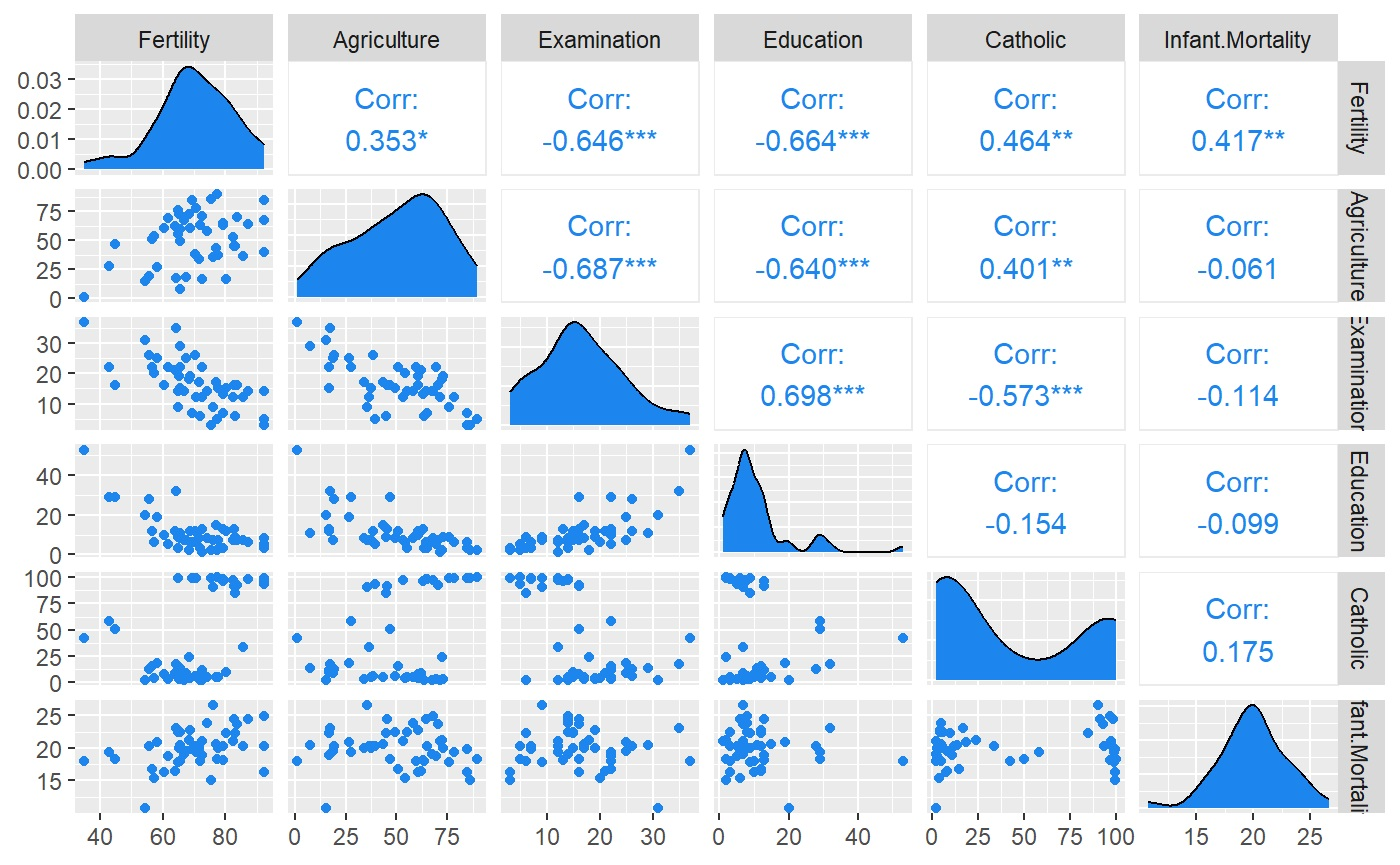
\includegraphics[width=1\textwidth]{images/3-2 corr}
	\caption{Matriz de Correlaciones Swiss.}
	\label{fig:corr2}
\end{figure}

En la figura 3.1 podemos observar que las variables tienen algún tipo de correlación lineal entre ellas. Si bien esta relación no es muy fuerte, consideramos que dichos valores no son despreciables. En resumen, determinamos que la distancia Euclídea no es la mejor manera de comparar las provincias entre sí, y que podría existir otro método mejor para realizar la comparación entre provincias.

\subsection{Tercer punto}

\textbf{Consigna:} Buscar la presencia de datos atípicos mediante la distancia de Mahalanobis. Comentar los resultados obtenidos.

Para buscar la presencia de datos atípicos lo primero que hicimos fue calcular la distancia de Mahalanobis. Luego, establecemos los puntos de corte utilizando la distribución de chi cuadrado con 6 grados de libertad para distintos niveles de significación ($0.90$, $0.95$ y $0.99$).  Los resultados de valores atípicos obtenidos se encuentran en la tabla 8.

\begin{table}[H]
	\centering
		\begin{tabular}{||l | c ||}
			\hline
			\hline
			Nivel de significación & Valor atípico\\
			\hline			
			\hline
			0.90 & Geneve, La Vallee, Porrentruy, Sierre, Neuchatel, Rive Droite\\
			\hline
			0.95 & Geneve, La Vallee, Porrentruy\\
			\hline
			0.99 & Geneve\\
			\hline
			\hline
		\end{tabular}
		\caption{Valores atípicos según la distancia de Mahalanobis con varios niveles de significancia.}
	\label{tab:table-punto-3-3}
\end{table}

\section{Ejercicio N° 4}
El Departamento de Psicología de una universidad ubicada en una ciudad céntrica realizó un estudio sobre la asistencia a clases teóricas no obligatorias dependiendo de la localidad de residencia del estudiantado. Para tal fin, se seleccionaron 40 estudiantes en la Ciudad A, 40 estudiantes en la Ciudad B y 40 estudiantes en la Ciudad C, y se contabilizó la cantidad de clases a las que cada uno/a asistió. Los resultados obtenidos se muestran en la siguiente tabla.

\begin{table}[H]
	\centering
		\begin{tabular}{|| c | c | c ||}
			\hline
			\hline
			Ciudad A & Ciudad B & Ciudad C\\
			\hline
			\hline		
			11 & 13 & 6\\
			\hline
			14 & 10 & 7\\
			\hline
			7 & 12 & 3\\
			\hline
			15 & 7 & 5\\
			\hline
			11 & 5 & 9\\
			\hline
			13 & 10 & 6\\
			\hline
			11 & 10 & 1\\
			\hline
			16 & 16 & 6\\
			\hline
			10 & 9 & 0\\
			\hline
			15 & 7 & 2\\
			\hline
			18 & 7 & 5\\
			\hline
			12 & 2 & 6\\
			\hline
			9 & 6 & 11\\
			\hline
			9 & 9 & 6\\
			\hline
			10 & 9 & 7\\
			\hline
			10 & 8 & 0\\
			\hline
			15 & 8 & 5\\
			\hline
			10 & 10 & 7\\
			\hline
			14 & 3 & 5\\
            \hline
            10 & 6 & 4\\
            \hline
            10 & 5 & 7\\
            \hline
            12 & 2 & 4\\
            \hline
            14 & 9 & 2\\
            \hline
            12 & 3 & 8\\
            \hline
            15 & 4 & 9\\
            \hline
            7 & 5 & 6\\
            \hline
            13 & 10 & 1\\
            \hline
            6 & 8 & 4\\
            \hline
            10 & 5 & 7\\
            \hline
            15 & 9 & 7\\
            \hline
            20 & 10 & 8\\
            \hline
            10 & 8 & 9\\
            \hline
            13 & 13 & 7\\
            \hline
            10 & 10 & 5\\
            \hline
            6 & 0 & 1\\
            \hline
            14 & 2 & 6\\
            \hline
            8 & 1 & 9\\
            \hline
            10 & 1 & 4\\
            \hline
            8 & 0 & 7\\
            \hline
            11 & 4 & 16\\
            \hline
			\hline
		\end{tabular}
		\caption{Tabla de asistencia a clases teóricas no obligatorias.}
	\label{tab:tabla-punto-4}
\end{table}

\subsection{Primer punto}

\textbf{Consigna:} Armar un \textit{data frame} en \textit{R} con los datos de la tabla anterior, creando dos variables: una que represente la cantidad de asistencias a las clases teóricas no obligatorias y otra que represente la localidad de residencia. ¿Qué tipo de variable es cada una?

Parte del data frame creado se puede visualizar en la tabla 10.

\begin{table}[H]
	\centering
		\begin{tabular}{|| c | c ||}
			\hline
			\hline
			Ciudad & Asistencia\\
			\hline
			\hline		
			A & 11\\
			\hline
			A & 14\\
			\hline
			B & 7\\
            \hline
            C & 5\\
            \hline
            .. & ..\\
            \hline
			\hline
		\end{tabular}
		\caption{Variables sobre la asistencia a clases teóricas no obligatorias según la localidad.}
	\label{tab:tabla-punto-4-1}
\end{table}

La variable ciudad es de tipo categórica y la variable Asistencia es de tipo numérica.

\subsection{Segundo punto}

\textbf{Consigna:} Analizar los datos de la muestra mediante gráficos y medidas estadísticas descriptivas. ¿Se observan diferencias en los valores promedios por localidad?

\begin{table}[H]
	\centering
		\begin{tabular}{||l || c | c | c | c ||}
			\hline
			\hline
			Ciudad & Media & Mediana & Rango & Desvío Estándar\\
			\hline			
			\hline
			A-B-C & 8.0 & 8.0 & $0-20$ & 4.22\\
			\hline
			A & 11.6 & 11.0 & $6-20$ & 3.16\\
			\hline
			B & 6.9 & 7.5 & $0-16$ & 3.84\\
			\hline
			C & 5.7 & 6.0 & $0-16$ & 3.13\\
			\hline
			\hline
		\end{tabular}
		\caption{Medidas estadísticas descriptivas.}
	\label{tab:table-punto-4-2}
\end{table}

\begin{figure}[H]
	\centering
	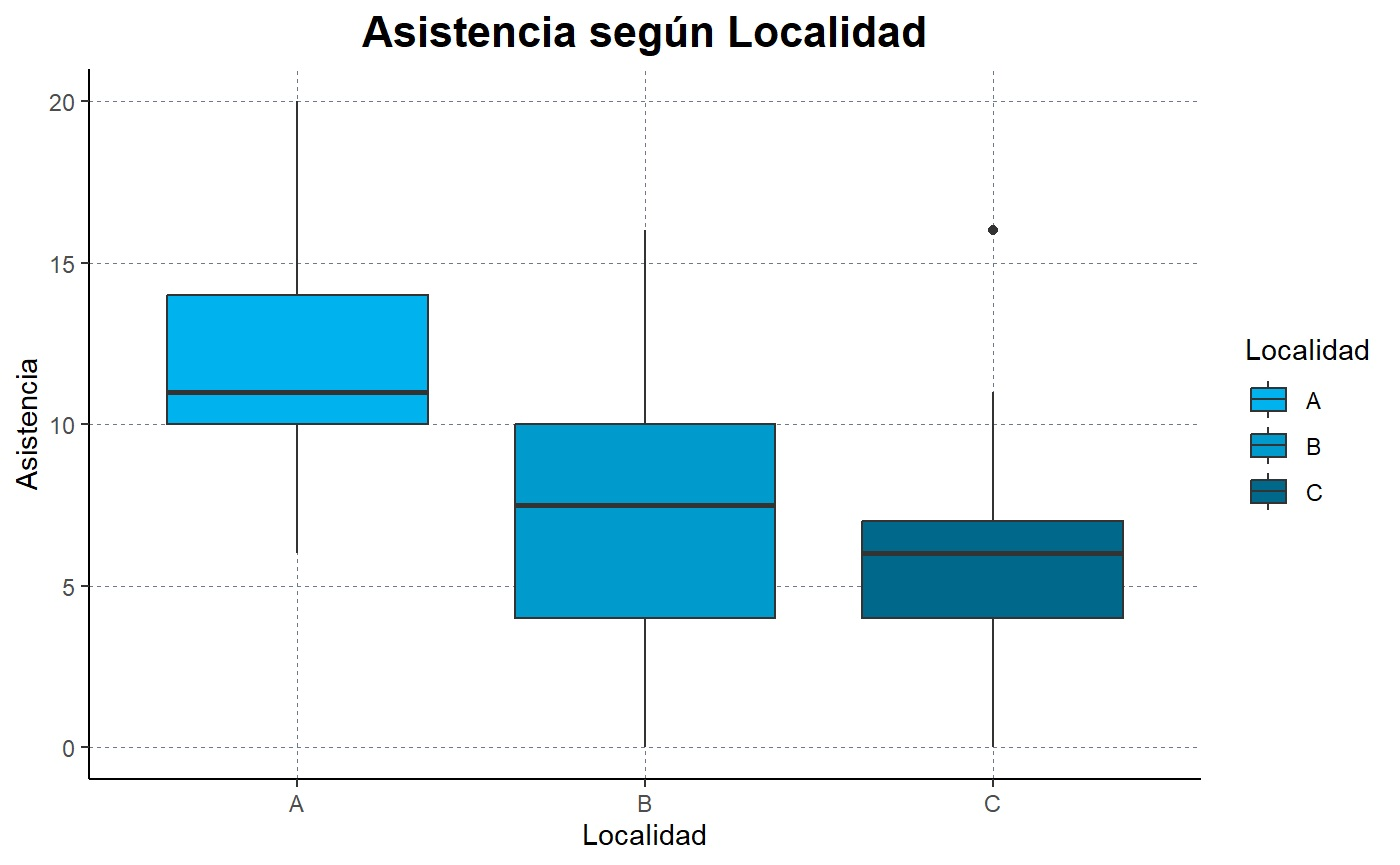
\includegraphics[width=0.8\textwidth]{images/4-2 box}
	\caption{Boxplot de Asistencia según Localidad.}
	\label{fig:box3}
\end{figure}

Observando la tabla 11 y la figura 4.1, podemos determinar que la ciudad A tiene un mayor promedio de asistencia a clases teóricas no obligatorias. Además, las ciudades B y C tienen valores relativamente parecidas, pero la B tiene un mayor desvío estándar. Por otro lado, la ciudad C cuenta con un valor atípico.

Ademas, analizando el gráfico se puede ver que los valores de la caja de la ciudad A, no llegan a superponerse con los valores de las otras dos ciudades, siendo esta la que se encuentra con los valores mas altos.


\subsection{Tercer punto}

\textbf{Consigna:} Realizar un test ANOVA para comparar las medias de las 3 poblaciones. Plantear las hipótesis nula y alternativa del test, informar los resultados obtenidos y la decisión tomada.

Para realizar el test de ANOVA, primero realizamos los test de normalidad y de homocedasticidad. La independencia suponemos que se cumple, ya que los individuos que fueron analizados en cada ciudad no son los mismos. 

La hipótesis nula para el test de ANOVA es: $h_0=\mu_A=\mu_B=\mu_C$ mientras que la alternativa es que existe al menos un par $i\neq j$ tal que $\mu_i \neq \mu _j$ significativamente.

En primer lugar, analizamos la normalidad de los datos de asistencia a partir de un gráfico de qqplot. Ademas, realizamos un test de Lilliefors para confirmar si los datos corresponden a una distribución normal. Utilizamos este test, y no el de Shapíro-Willk, porque estamos trabajando con más de 50 datos.

\begin{figure}[H]
	\centering
	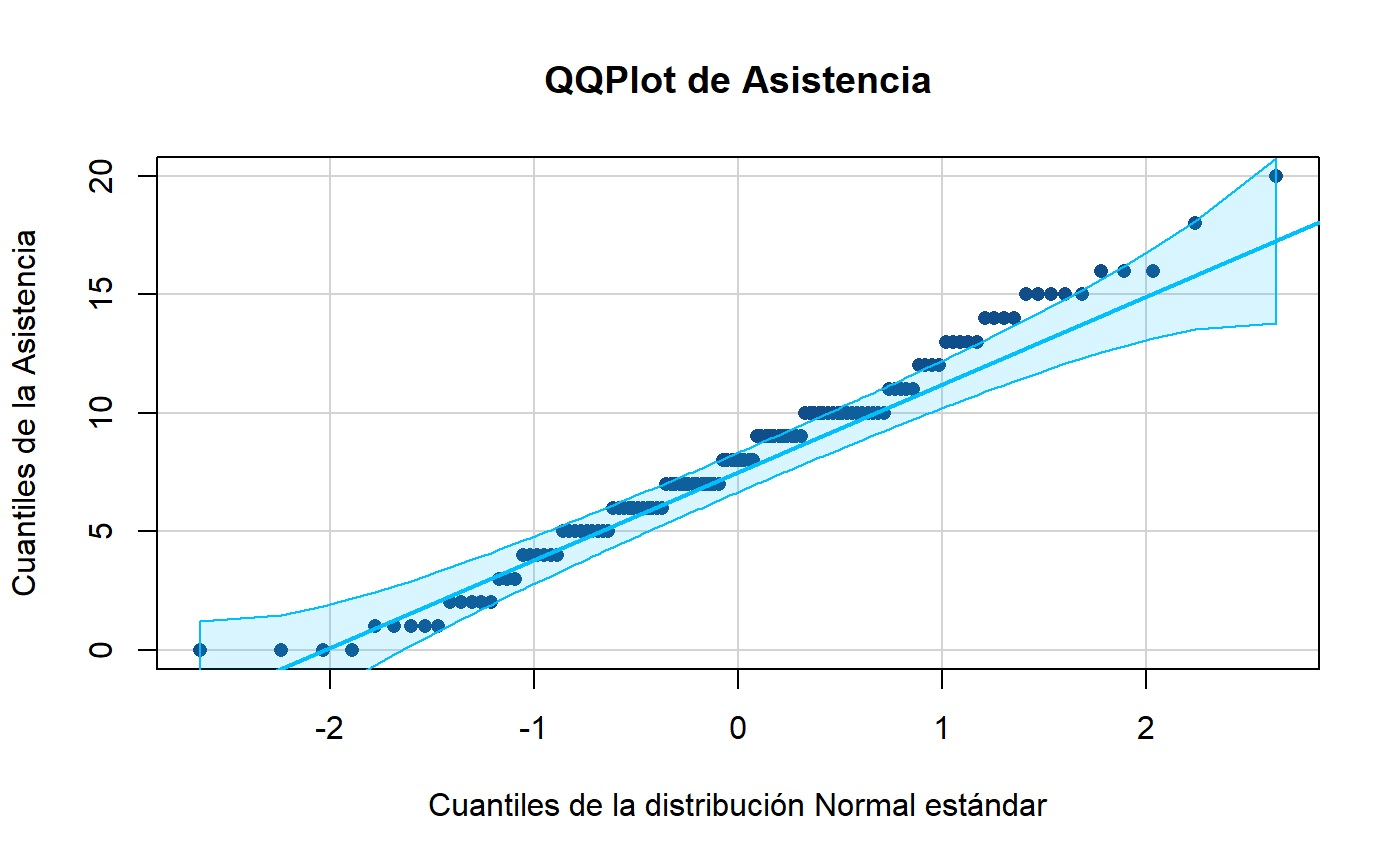
\includegraphics[width=0.8\textwidth]{images/4-3 qq}
	\caption{QQPlot de Asistencia.}
	\label{fig:qq}
\end{figure}

El QQPlot de la figura 4.2 nos dio bastante normal, siendo que los puntos se encuentran en el rango, con algunos fuera de este en el margen superior derecho. Por otro lado, al realizar el test de Lilliefors, nos dio un p-value menor al nivel de significancia, por lo cual determinamos que el conjunto no sigue una distribución normal. A pesar de esto, decidimos continuar con el análisis, ya que suponemos que los resultados obtenidos no se encuentran tan significativamente fuera del rango de normalidad. 

Continuamos con el análisis de homocedasticidad de los datos, para esto utilizamos el test de Levene. En nuestro caso nos dio $0.15$ por ende no rechazamos la hipótesis nula que supone la igualdad de las varianzas en los grupos.

Procedemos a realizar el test de ANOVA sobre la asistencia según la ciudad. Luego de obtener los resultados, calculamos el tamaño del efecto para compararlos con los niveles de clasificación más comunes. 

En la tabla 12 podemos ver los indicadores del test de ANOVA.

\begin{table}[H]
	\centering
		\begin{tabular}{||l | c||}
			\hline
			\hline
			Indicadores & Resultado\\
			\hline			
			\hline
			Grado de Libertad & $2$\\
			\hline
			Estadístico F & $33.72$\\
			\hline
			P-Value & $2.74e^{-12}$\\
			\hline
			Tamaño del Efecto & $0.36$\\
			\hline
			\hline
		\end{tabular}
		\caption{Resultados de ANOVA.}
	\label{tab:table-punto-4-3}
\end{table}

El P-Value obtenido es más bajo que el corte usual de $0.05$. El tamaño del efecto nos dio mayor que el nivel de clasificación de $0.14$, por lo tanto deducimos que la varianza de la asistencia se encuentra explicada en gran medida por el tipo de ciudad en la que se encuentra. A partir de los resultados obtenidos, podemos concluir que existen diferencias significativas entre las medias de las asistencias en las distintas ciudades.

\subsection{Cuarto punto}

\textbf{Consigna:} Si se han obtenido diferencias significativas entre las localidades, determinar cuáles son esas diferencias utilizando el test de Tukey.


\begin{table}[H]
	\centering
		\begin{tabular}{||l | c | c | c | c ||}
			\hline
			\hline
			Intersecciones & Diff & Lower & Upper & P-Value\\
			\hline			
			\hline
			B-A & -4.7 & -6.5 & -2.8 & 0\\
			\hline
			C-A & -5.9 & -7.7 & -4.1 & 0\\
			\hline
			C-B & -1.2 & -3.0 & -0.6 & 0.258\\
			\hline
			\hline
		\end{tabular}
		\caption{Resultados de Tukey.}
	\label{tab:table-punto-4-3}
\end{table}

A partir de los resultados obtenidos en la tabla 13, podemos concluir que existen diferencias estadísticamente significativas en las medias de las asistencias entre las ciudades A-B y A-C, donde los valores del P-Value son menores a $0.05$.


\end{document} % This is the end of the document
